\documentclass[]{article}
\usepackage[spanish]{babel} 
\usepackage{amsmath} 
\usepackage[colorlinks=true]{hyperref}
\usepackage{enumitem} 
\usepackage{graphicx}   
\usepackage[a4paper,top=2.5cm,bottom=2.5cm,left=2cm,right=2.5cm]{geometry} 
\usepackage[]{subfigure}
\usepackage[]{multicol}
\setlength{\columnsep}{1cm}
\usepackage[]{hyperref}
%\usepackage[maxbibnames=99, sorting=none]{biblatex}
\usepackage{amssymb}
\usepackage[]{txfonts}

%\usepackage[authoryear]{natbib}
\newenvironment{Figura}
{\par\medskip\noindent\minipage{\linewidth}}
{\endminipage\par\medskip}


\title{Electromagnetismo} 
\author{Noemí de la Peña, Benjamín Opazo, Martina Contreras \\ \\
\textit{ Departamento de Física, Universidad de Concepción, Concepción, Chile. }}
\date{} 





%==================================================================================
\begin{document}
\maketitle 

\begin{abstract}
  En este laboratorio se llevaron a cabo 4 experimento relacionados con los circuitos eléctricos, donde se hizo varear el voltaje de entrada para estudiar la variación de la intensidad de corriente en cada circuito.
Los circuitos utilizados fueron: Conductor metálico, Filamento de ampolleta de linterna, Diodo semiconductor común y Diodo emisor de luz (DEL o LED).
Donde se concluye que la cantidad de intensidad de corriente soportada por cada circuito depende de los materiales que componen.
\end{abstract}



%========Introducción=============
\section*{Introdución}
Los primeros pasos para la creación de circuitos eléctricos fueron dada por el químico Alessandro Volta y la creación de la primera pila moderna. Ese fue el punto de partida básico para la   utilización práctica de la energía eléctrica pasando a través de circuitos para cumplir diferentes finalidades.
Más tarde, hacia 1826, sería Georg Simon Ohm quien sentará las bases del estudio de la circulación de las cargas eléctricas en el interior de materias conductoras y formula la ley que relaciona las tres magnitudes más importantes: voltaje, intensidad y resistencia.
En este informe, primero definiremos conceptos claves para entender que es un circuito, tales como: Voltaje, Intensidad y resistencia. Luego presentaremos los materiales y procedimientos utilizados y un análisis para cada circuito utilizado, para concluir con lo que hemos aprendido en este laboratorio.


%==============Marco teorico============
\section*{Marco teórico}

  \textbf{La Corriente eléctrica,} expresada como un flujo de partículas, se escribe:
  \begin{align*}
    I = \int_{A} J\cdot  dS
  \end{align*}
  donde: \\
    $J = \sum_{i} n_i \, q_i \langle v_i\rangle$ es el \textbf{vector densidad de corriente}, la cual expresa
    la contribución de los eventuales varios portadores de carga participantes en el proceso de condución eléctrica,
    dependiendo de la clase de material de que se trate. En la conducción metálica, los portadores son electrones solamente, entonces,
    \begin{align*}
      J = n_i \, e\mu E
    \end{align*} 
  donde $n, e, \mu$ expresan la concentración (número/volumen), la carga y la movilidad de los electrones, respectivamente,
  cuando hay aplicado un campo eléctrico \textbf{E}. Definimos $\sigma = n_i \, e\mu$ como la conductividad del material conductor en estudio y 
  $\rho = \frac{1}{\sigma}$ su resistividad. \\

  Para un trozo de conductor cilíndrico, de área transversal $A$ y longitud $l$, su resistencia eléctrica $R$ queda expresada
  por: 
  \begin{align*}
    P = I^2 \, R = V \, I = \frac{V^2}{R}
  \end{align*} 
  Esta relación expresa la rapidez con que se fectuá la transformación o potencia desarrollada. \\
  
  La teoría de conducción eléctrica en semiconductores, considera dos clases de portadores de carga, electrones
  con carga $(-e)$ y huecos con carga $(+e)$. Ambos tipos tienen igual concentración cuando el semiconductor está en estado
  puro (intrínseco). Por métodos físico-químicos se pueden incorporar átomos de otros elementos ("impurezas") que permiten
  hacer que una u otra de las concentraciones de portadores predomine. Si predominan los portadores de carga $(-)$ se habrá 
  obtenido un semiconductor tipo $n$ y de tipo $p$, llamada unión $p - n$. Las propiedades de una unión $p-n$ se verán reflejadas en la curva característica
  I vs V de los diodos.





%=========Materiales===============
\section*{Materiales}

\begin{multicols*}{2}
  \begin{itemize}
    \item Conductor metálico (fino alambre de metal).
    \item Filamento de ampolleta de linterna.
    \item Diodo semiconductor común.
    \item Diodo emisor de luz (DEL o LED).
    \item Una fuente de poder electrónica (FPE).
    \item Dos multímetros digitales.
    \item Siete cables de conexión.
  \end{itemize}
\end{multicols*}
%================Procedimiento=================================

1.- Ubicamos los selectores de M1 y M2 en 40(DCV) y 2 (DCA), respectivamente. Ahora, conectamos M1, y M2.
Instalamos como elemento X el \textbf{conductor metálico}, conectándolo entre P y Q. La corriente máxima que 
se hará circular será de 0.50 A. 
Luego, hacemos 10 medidas en el rango (0.00 - 0.50)(A) para cada polaridad. Una vez que tomamos los datos, desconectamos
el terminal \textbf{(+)} de la \textbf{FPE} y accionamos el control para volver a $0 V$ en la fuente. \\


2.- Cambiamos el elemento X, instalando ahora la \textbf{ampolleta de la linterna.} Volvemos a conectar el terminal $(+)$ de la FPE. 
Para no dañar su filamento, conviene seleccionar un rango apropiado de corrientes. Se nos recomienda utilizar los
siguientes valoresen la escala de $400 mA$ (DCA) de M2: 20; 40; 60; 80; 100; 120; 160; 180; 200. Mantenemos M1 en 
su escala. Aquí también efectuamos la inversición de polaridad, para cada valor de corriente. Denuevo, al finalizar la serie,
desconectamos el terminal (+) y retornamos a $0 (V)$ la FPE.

3.- A continuación, cambiamos el elemento X, instalando el diodo \textbf{semiconductor común.} Reinstalamos la conexión
del terminal $(+)$ de la FPE. Ahora, trabajaremos separadamente las polaridades directa e inversa. Con polarizacion directa,
ajustamos los siguientes valores de corriente en la escala de 2 A (DCA): 0.050; 0.080; 0.100; 0.120; 0.130;
0.140; 0.160; 0.200; 0.250; 0.300; 0.350; 0.400. Iniciamos el control de voltaje de manera cuidadosa, desde 0.00 V hasta
0.60 V. De ahí en adelante extremamos las precauciones ajustando sólo con el control fino. Tratamos de definir el llamado
voltaje de arranque del diodo, donde se hace bruscamente el conductor. Luego, cambiamos a polaridad inversa
y exploramos hasta donde sea posible; valores altos de voltajes son permitidos, en tanto la corriente se mantenga baja. Efectuamos 10 
medidas para cada polaridad. Finalmente, desconectamos el terminal (+) y retornamos a 0 (V) la salida de la fuente.


4.- Instalamos el diodo emisor de luz. Restauramos la conexión (+) de la fuente y comenzamos a incrementar el voltaje
hasta 1.50 V en una primera etapa. Luego, prestamos más atención a los valores de corriente ajustando con el control 
fino de voltaje 10 pares de valores $I^{+}$, $V^{+}$ con corrientes comprendidas en el rango: 0.20 (mA), hasta 5.00 (mA)
en la escala de 40 (mA) (DCA). Luego, tratamos de ubicar el punto de encendido del LED, visualmente y anotamos dicho valor; efectuamos
10 medidas $I^{+}$, $V^{+}$ para la polaridad. Además, realizamos mediciones con polaridad inversa con el LED.











%============Análisis==========================================================
\section*{Análisis}

\begin{table}
  \centering
  \begin{tabular}{|c|c|c|c|c|} \hline
    dato    &   $V^{+}$ [v]  &    $I^{+}$[A]  &   $V^{-}$ [v]  &    $I^{-}$ [A]  \\ \hline
    1       & 0.02 &0.01   &-0.56 &-0.05 \\ \hline
    2      &0.28  &0.02     &-0.74 &-0.07 \\ \hline
    3      &0.45  &0.03     &-1.35 &-0.12 \\ \hline
    4       &0.73  &0.07    &-1.76 &-0.17 \\ \hline
    5       &0.99  &0.09    &-2.23 &-0.22 \\ \hline
    6       &1.42  &0.14    &-2.66 &-0.27 \\ \hline
    7       &2.63  &0.26    &-3.42 &-0.35 \\ \hline
    8       &3.71  &0.37    &-3.97 &-0.41 \\ \hline
    9       &4.13  &0.42    &-4.29 &-0.44 \\ \hline
    10       &4.82  &0.49   &-4.92 &-0.5 \\ \hline

  \end{tabular}
  \caption{\label{tab: transitor} Conductor metálico}
\end{table}






\begin{table}
  \centering
  \begin{tabular}{|c|c|c|c|c|} \hline
    dato    &   $V^{+}$ [v]  &    $I^{+}$[A]  &   $V^{-}$ [v]  &    $I^{-}$ [A]  \\ \hline
    1& 0.10 &0.01 &-0.05& 0.00 \\ \hline
    2&0.31 &0.02  &-0.09& 0.01 \\ \hline
    3&0.71 &0.03 &-0.18& 0.02 \\ \hline
    4&0.81 &0.04 &-0.39& 0.03 \\ \hline
    5&1.09 &0.05 &-0.89& 0.04 \\ \hline
    6& 1.49 &0.06 &-1.15& 0.05 \\ \hline
    7& 1.72 &0.07 &-1.60& 0.06 \\ \hline
    8& 2.01 &0.08 &-2.03& 0.07 \\ \hline
    9& 2.90 &0.09  &-2.56& 0.08 \\ \hline
    10& 3.64 &0.10 &-3.26& 0.10 \\ \hline
    
    
  \end{tabular}
  \caption{\label{tab: ampolleta} Ampolleta de linterna. }
\end{table}



\begin{table}
  \centering
  \begin{tabular}{|c|c|c|c|c|} \hline
    dato    &   $V^{+}$ [v]  &    $I^{+}$[A]  &   $V^{-}$ [v]  &    $I^{-}$ [A]  \\ \hline
    1&0.67& 0.00&     -0.40& 0.00\\ \hline
    2&0.68& 0.00&     -1.98& 0.00\\ \hline
    3&0.70& 0.00&     -4.08& 0.00\\ \hline
    4&0.71& 0.00&     -6.53& 0.00\\ \hline
    5&0.72& 0.00&     -7.35& 0.00\\ \hline
    6&0.73& 0.01&     -8.41& 0.00\\ \hline
    7&0.74& 0.02&     -9.23& 0.00\\ \hline
    8&0.75& 0.03&     -10.08& 0.00\\ \hline
    9&0.76& 0.04&     -11.41& 0.00\\ \hline
    10&0.76& 0.04&     -12.62& 0.00 \\ \hline
    
    
  \end{tabular}
  \caption{\label{tab: diodo-comun} Diodo semiconductor común.}
\end{table}


\begin{table}
  \centering
  \begin{tabular}{|c|c|c|c|c|} \hline
    dato    &   $V^{+}$ [v]  &    $I^{+}$[A]  &   $V^{-}$ [v]  &    $I^{-}$ [A]  \\ \hline
    1&0.00& 0.00&     -0.93	&0.00\\ \hline
    2&1.43& 0.00&     -2.17	&0.00\\ \hline
    3&1.80& 0.00&     -3.42	&0.00\\ \hline
    4&2.40& 0.01&     -4.42	&0.00\\ \hline
    5&2.56& 0.01&     -5.62	&0.00\\ \hline
    6&2.65& 0.02&     -7.46	&0.00\\ \hline
    7&2.80& 0.02&     -8.84	&0.00\\ \hline
    8&2.95& 0.02&     -10.21	&0.00\\ \hline
    9&3.01& 0.03&     -11.00	&0.00\\ \hline
    10&3.35& 0.04&     -12.22	&0.00\\ \hline
    
    
  \end{tabular}
  \caption{\label{tab: emisor-luz} Diodo emisor de luz.}
\end{table}

\begin{figure}
  \centering
  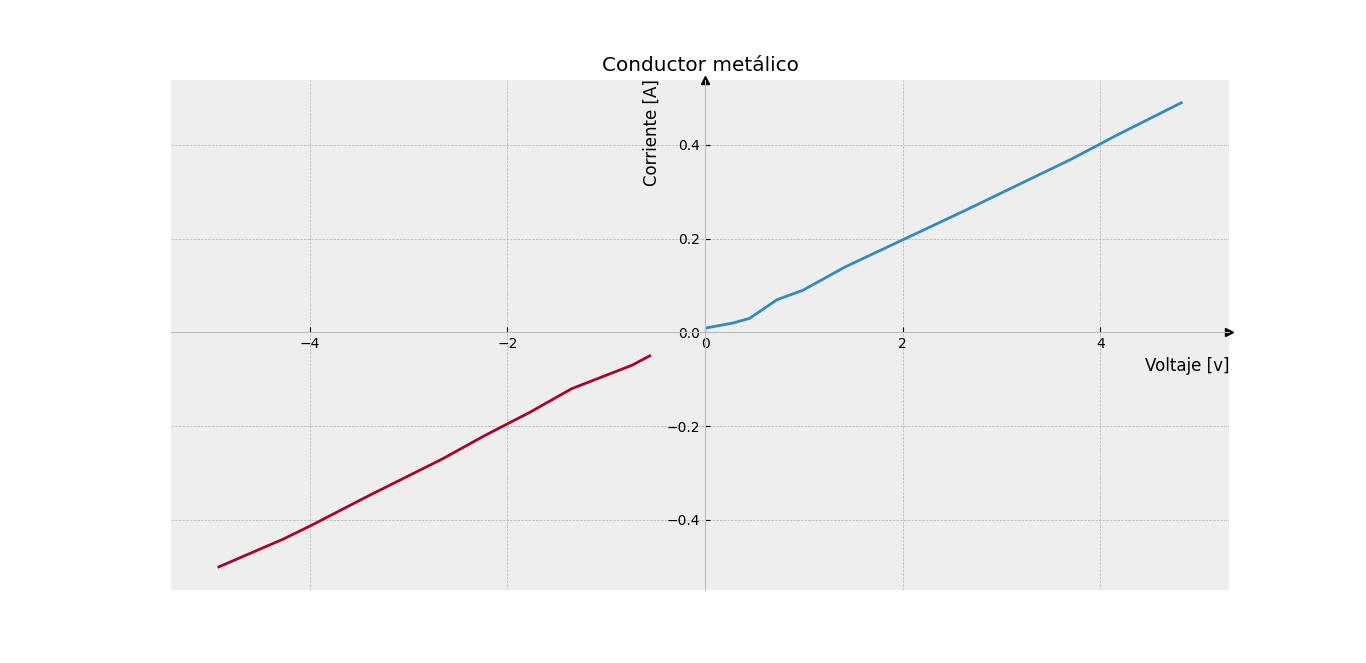
\includegraphics[width=12cm, height=8cm]{img/Figure_2.png}
  \caption{\label{fig: fig-conductor}Gráfico de conductor metálico.} 
\end{figure}

\begin{figure}
  \centering
  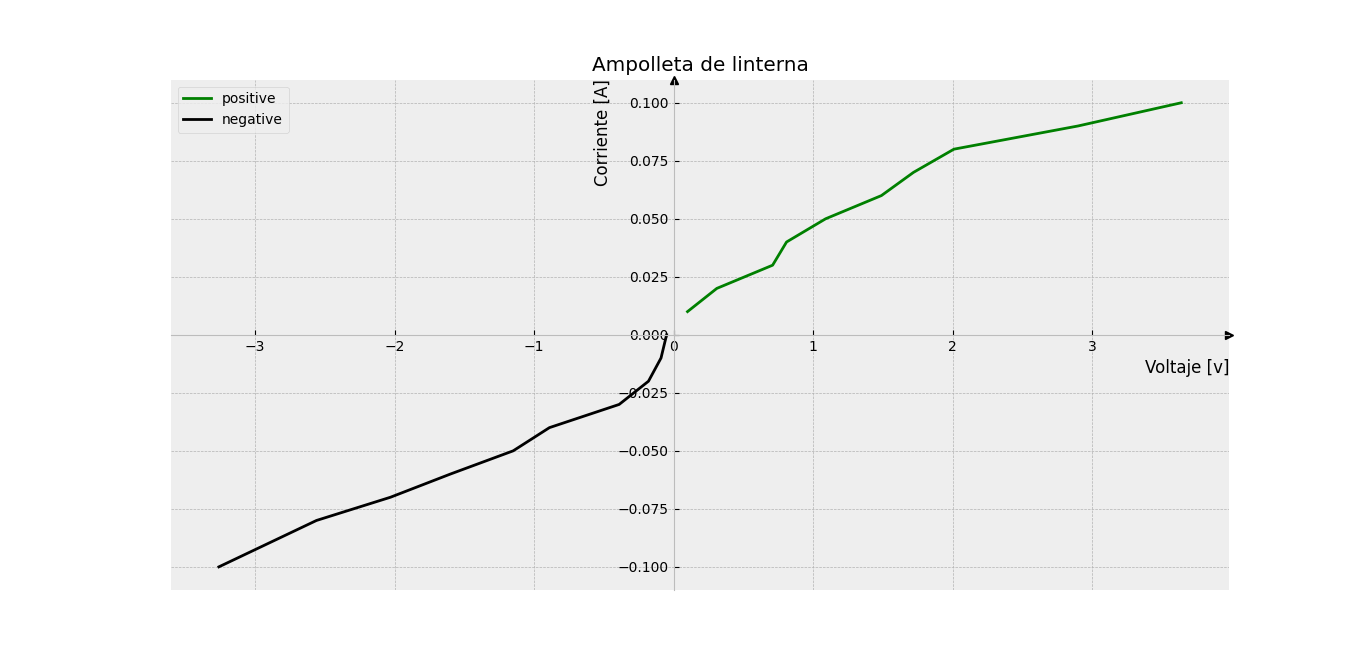
\includegraphics[width=12cm, height=8cm]{img/Figure_1.png}
  \caption{\label{fig: fig-ampolleta}Gráfico ampolleta de linterna.} 
\end{figure}

% \begin{figure}
%   \centering
%   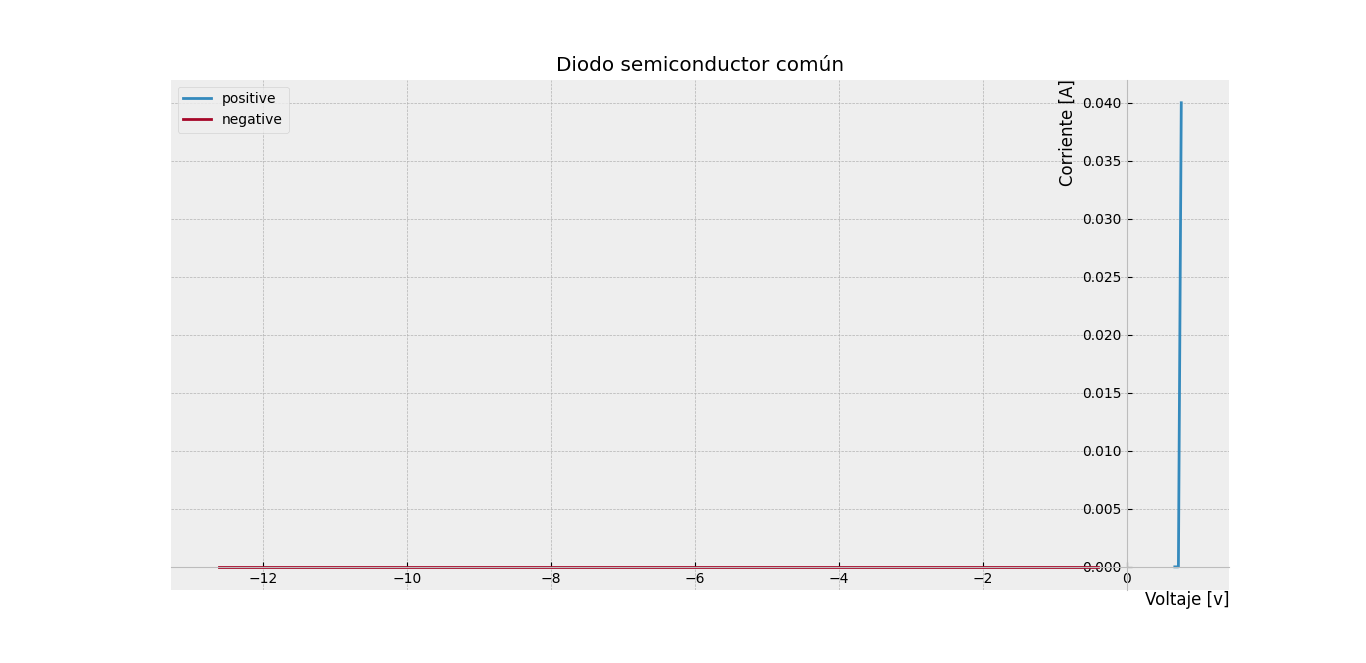
\includegraphics[width=12cm, height=8cm]{img/Figure_3.png}
% \end{figure}

%============Conclusión========================================================
\section*{Conclusión}


\begin{thebibliography}{5}
  \bibitem{Ley-de-Lorentz}  Ley de Lorentz. (s. f.). Fisicalab. Recuperado 7 de octubre de 2022, 
  de \url{https://www.fisicalab.com/apartado/ley-de-lorentz}
  \bibitem{Ley-de-Ampere}Ley de Ampère. (s. f.). Fisicalab. Recuperado 8 de octubre de 2022, 
  de \url{https://www.fisicalab.com/apartado/ley-de-ampere}
  \bibitem{Ley-de-Faraday} \textbf{D. Halliday; R. Resnick; K. S. Kane.} \textit{Física Vol. 2.} (Cap.36), Compañía Editorial Continental, S.A. de C.V. 3º Edición, 1994
  \bibitem{Corrientes-de-Foucault} Eddy Current, que es y como detectarla. - Frigochiller. (2020, 31 marzo). Frigochiller - Mantenimiento y reparacion de Chillers. Recuperado 8 de octubre de 2022, 
  de \url{https://frigochiller.com/corriente-de-foucault/}
\end{thebibliography}




\end{document}